\chapter{Ramond-Neveu-Schwarz超弦}
本章使用超对称共形场论(SCFT)的方法介绍世界面超对称的RNS超弦理论。更多细节详见\cite{Green:2012oqa,Green:2012pqa}。
\section{世界面超场}
考虑世界面超对称,Polyakov作用量\ref{eq:2.2}中为$X$引入世界面自旋$\frac12$超伴场$\Psi$,为$\gamma$引入世界面自旋$\frac32$超伴场$\chi$,他们都是世界面上的二维旋量。在世界面Wick转动后,RNS超弦作用量为\footnote{$\rho$是二维gamma矩阵。}:
\begin{equation}
	\begin{aligned}
		S_{\mathrm{RNS}}[X,\Psi,g,\chi]=&\frac1{4\pi}\int\mathrm{d}^2\sigma\sqrt{-g}\Big[-\frac1{\alpha^{\prime}}g^{\alpha\beta}\partial_\alpha X^\mu\partial_\beta X_\mu+\overline{\Psi}^\mu\rho^\alpha\nabla_\alpha\Psi_\mu\\&+(\overline{\chi}_\alpha\rho^\beta\rho^\alpha\Psi^\mu)\Big(\frac1{\sqrt{2\alpha^{\prime}}}\partial_\beta X_\mu+\frac18\overline{\chi}_\beta\Psi_\mu\Big)\Big]
	\end{aligned}
\end{equation}
对于闭弦,上述作用量的超对称荷有左右模部分,所以实际上是$\mathcal{N}=2$超对称,而超弦只有左模有贡献,所以是$\mathcal{N}=1$超对称。后面将会看到他们低能极限下的谱分别是$\mathcal{N}=2$超引力以及$\mathcal{N}=1$超对称Yang-Mills理论。

现在$\mathrm{diff}\times\mathrm{Weyl}$不变性被提升为$\mathrm{Super\mbox{-}diff}\times\mathrm{Super\mbox{-}Weyl}$不变性,类似\ref{eq:2.30}取等温坐标到共形规范下消去$g$,这里我们可以取超共形规范消去$\chi$,并且将Majorana旋量\footnote{二维情况下总可以选取$\rho$的实表示从而要求$\Psi$为实的,这在二维情况下意味着是Majorana旋量}$\Psi$分解成左右手Weyl旋量$\psi/\bar\psi$。最终得到世界面上的超对称共形场论的物质项:
\begin{equation}
	S=\frac{1}{2\pi}\int\mathrm{d}^2z\left(\frac{2}{\alpha^{\prime}}\partial X^\mu\overline{\partial}X_\mu+\psi^\mu\overline{\partial}\psi_\mu+\overline{\psi}^\mu\partial\overline{\psi}_\mu\right)
\end{equation}
同时可以引入玻色鬼场$bc$以及费米鬼场$\beta\gamma$:
\begin{equation}
	S_{\mathrm{gh}}=\frac{1}{2\pi}\int\mathrm{d}^2z\left(b\overline{\partial}c+\overline{b}\partial\overline{c}+\beta\overline{\partial}\gamma+\overline{\beta}\partial\overline{\gamma}\right)
\end{equation}
共形变换以及相应的超共形变换的能动张量为:
\begin{equation}
	\label{eq:3.4}
	\begin{gathered}
		\frac{\delta S_m}{\delta g}\sim T^\mathrm{m}(z)=-\frac{1}{\alpha^{\prime}}:\partial X\cdot\partial X:-\frac{1}{2}:\psi\cdot\partial\psi:\\
		\frac{\delta S_m}{\delta\chi}\sim G^\mathrm{m}(z)=i\sqrt{\frac{2}{\alpha^{\prime}}}\psi^\mu\partial X_\mu
	\end{gathered}
\end{equation}
由于$g,\chi$都没有动力学,$T^m,G^m$应当为$0$类似\ref{eq:2.22}作为约束出现。另外$bc\beta\gamma$鬼场总共对中心荷贡献$-15$,而玻色场贡献$D$,费米场贡献$\frac{D}{2}$,所以共形反常消去必须要求:
\begin{equation}
	\boxed{D_{\mathrm{super}}=10}
\end{equation}

后面的讨论主要针对左模。类似开弦边界条件\ref{eq:2.9}的边界条件选取消去作用量泛函导数的边界项贡献,最终加倍技巧后体现为左右模相等\ref{eq:2.35}。而对RNS超弦,类似的条件会导致世界面超场左右模之间相差正负号,从而给出两种不同的超场模展开:
\begin{equation}
	\psi_{\mathrm{NS}}^\mu(z)=\sum_{r\in\mathbb{Z}+\frac{1}{2}}\psi_r^\mu z^{-r-\frac{1}{2}},\quad\psi_{\mathrm{R}}^\mu(z)=\sum_{n\in\mathbb{Z}}\psi_n^\mu z^{-n-\frac{1}{2}}
\end{equation}
世界面超场应当看作是在复平面的双覆盖黎曼面上定义。世界面超流$G$以及$\beta\gamma$鬼场同样可以分为NS和R两个部分,只是$z$的指数依赖要根据共形权重写。后面会看到$R$部分负责产生费米子,NS部分负责产生玻色子。对于闭弦,边界条件\ref{eq:2.8}变化为超场可以满足周期性或者反周期性。左右模部分可以分别处于NS,R部分,所以总共有四个部分。

最后来讨论一下费米物质场的真空。玻色场的真空由$\alpha^\mu_{n\geq 1}$湮灭的$\ket{0;p^\mu}$生成,其中$p^\mu\propto\alpha^\mu_0$用来标记真空动量$p^\mu$。类似的,费米物质场真空也由对应的湮灭算符产生:
\begin{equation}
	\psi_{r\geq\frac12}^\mu\left|0,p\right\rangle_{\mathrm{NS}}=0,\quad \psi_{n\geq1}^\mu\left|0,p\right\rangle_{\mathrm{R}}=0
\end{equation}
$\psi_0$类似$\alpha_0$既不是产生也不是湮灭算符,而是用于标记简并的真空态。不过$\psi_0$只存在于R部分真空,所以NS部分的真空依旧直接是$\ket{0}_{\mathrm{NS}}$,而且这也正是$\frac12$共形权的$\psi$场的$SL(2,\mathbb{C})$不变真空。注意到$\psi_0$之间满足:
\begin{equation}
	[\psi_0^\mu,\psi_0^\nu]=\eta^{\mu\nu}
	\xleftrightarrow{\Gamma\sim\sqrt{2}\psi_0} [\Gamma^\mu,\Gamma^\mu]=2\eta^{\mu\nu}
\end{equation}
也就是说R部分真空应当处于$SO(9,1)$的旋量表示也就是十维Clifford代数表示中,是具有$2^5=32$个分量的Dirac旋量$\left|A^{\prime}\right\rangle_{\mathrm{R}}=\left|A\right\rangle\oplus|\dot A\rangle$,现在考虑$G^m=0$的限制要求,类似\ref{eq:2.23},对R部分有:
\begin{equation}
	G^m_{n\geq0}\left|\mathrm{phys}\right\rangle_{\mathrm{R}}=\sum_{m\in\mathbb{Z}}\alpha_m\cdot\psi_{m-n}\left|\mathrm{phys}\right\rangle_{\mathrm{R}}=0
\end{equation}
这个时候由于\ref{eq:3.4}中$G^m$部分$\psi$与$\partial X$之间OPE正则,所以不需要引入类似\ref{eq:2.23}的正规排序常数\footnote{这其实也是因为鬼场和物质场对R真空的总真空能贡献为0。}。考虑$n=0$时类似$L_0=0$的质量在壳条件,物质场超流要求的在壳条件可以改写为下面的Dirac-Ramond方程:
\begin{equation}
	\left(p\cdot\Gamma+\frac{2\sqrt{2}}{\ell}\sum_{n=1}^\infty(\alpha_{-n}\cdot \psi_n+\psi_{-n}\cdot\alpha_n)\right)\left|\mathrm{phys}\right\rangle_{\mathrm{R}}=0
\end{equation}
上述方程对真空态退化为$p\cdot\Gamma\ket{0}=0$即Dirac方程。这一方程将每个Weyl分量从$16$缩减到$8$。后面GSO投影会对这一自由度再次进行修正。

NS真空是$SL(2,\mathbb{C})$不变真空,而R真空实际上可以看作是NS真空的激发态,自旋场\footnote{其本质来源于$\psi$的玻色化\cite{Blumenhagen:2013fgp,Schlotterer:2012zz},不过后续计算我们并不会过多使用$S_A$。}将这两个真空联系起来:
\begin{equation}
	\left|A^{\prime}\right\rangle_{R}=\lim_{z\to 0}S_{{A^{\prime}}}(z)\left|0\right\rangle_{NS},\quad 
	{}_R\left\langle A^{\prime}\right|=\lim_{z\to\infty}{}_{NS}\left\langle0\right|S_{{A^{\prime}}}(z)z^{D/8}
\end{equation}
$z^{D/8}$的出现是BPZ共轭的要求\cite{itocft},$S_A$的共形权为$\frac{D}{16}=\frac58$,其来自于R部分物质场真空能贡献,相应的NS部分物质场真空能贡献为0:
\vspace{1.5em}% 这里需要调
\begin{equation}
	\label{eq:3.12}
	a^{\mathrm{m}}_R=
	\eqnmarkbox[blue]{node1}{\frac{1}{24}c^{\mathrm{m}}}+
	\left(\eqnmark[red]{node2}{-\frac{1}{24}}+\tikzmarknode{node3}{\frac{1}{24}}\right)D=\frac{1}{16}D
\end{equation}
\annotate[yshift=1em]{right}{node1}{能动张量非主场,共形变换贡献}
\annotate[yshift=-0.5em]{below,left}{node2}{玻色场贡献}
\annotate[yshift=-1em]{below,label below}{node3}{费米场贡献}
\vspace{1em}
\section{正则量子化}
本节使用光锥量子化处理RNS超弦,好处是规范完全固定,只用讨论物质场,能方便看出粒子谱的超对称性\footnote{协变量子化可见\href{https://www.uu.se/en/department/physics-and-astronomy/research/theoretical-physics/oliver-schlotterer}{Oliver Schlotter的在线讲义}。}。后面再使用BRST量子化来构造协变的顶角算符,后面的讨论以开弦为例。

玻色场的光锥规范依旧和第\ref{chap:2}章的讨论相同,费米场NS部分的光锥规范有如下的简单形式:
\begin{equation}
	\psi^+ = 0
\end{equation}
R部分同上式一样,唯一不同是保留零模,用于生成简并R真空。而$\psi^-$部分同样也可以用横向振动激发描述。所以$\psi^\pm$不再拥有动力学,我们只需要关注横向振动激发。粒子谱由$\psi^i_\bullet,\alpha^i_\bullet$作用在R和NS真空上得到。

NS部分的质量谱可以从$L_0^m$最高权限制给出的在壳条件推出:
\begin{equation}
	\label{eq:3.14}
	\alpha^{\prime}m^2_{NS}=\sum_{n=1}^\infty\alpha_{-n}^i\alpha_n^i+\sum_{r=1/2}^\infty r\psi_{-r}^i\psi_r^i-\frac{1}{2}
\end{equation}
这里$-\frac12$来源于\ref{eq:3.12}类似的计算,注意还要加上鬼场的贡献,同理R部分有:
\begin{equation}
	\alpha^{\prime}m^2_{R}=\sum_{n=1}^\infty\alpha_{-n}^i\alpha_n^i+\sum_{n=1}^\infty n\psi_{-n}^i \psi_n^i
\end{equation}
不过从\ref{eq:3.14}能看出NS部分依旧存在快子态。
\section{GSO投影}
RNS形式只保证了世界面上的超对称性,而我们更应当要求保留十维靶空间的超对称性。这一点需要在量子化的基础上剔除一些态。定义如下的G宇称算符:
\begin{equation}
\begin{aligned}
		G_{NS}&=(-1)^{F+1}=(-1)^{\sum_{r=1/2}^\infty \psi_{-r}^i\psi_r^i+1}\\
	G_R&=\Gamma_{11}(-1)^{\sum_{n=1}^\infty \psi_{-n}^i\psi_n^i}
\end{aligned}
\end{equation}
其中$\Gamma_{11}=\Gamma_{0}\Gamma_{1}\ldots\Gamma_{9}$。GSO投影要求NS部分的态满足$G_{NS}=+1$,显然快子态不满足这一要求,所以被剔除了,基态变为无质量矢量玻色子激发$\psi^i_{-1/2}\ket{0}_{NS}$。对于R部分,为了要求处于$G_R$本征态,则是要求剔除掉一般的手征。也就是说如果我们选取$\ket{\alpha;+}_R$\footnote{其实记号$\alpha$就已经表明了$\Gamma_{11}=+1$,这里后面加个$+$只是为了符号更加清晰。}作为基态,那么投影到$G_R=+1$,反之投影到$G_R=-1$。也就是说在GSO投影下,R部分基态从$8\oplus 8$破缺成了仅含一个手征$8$。对于开弦来说,取左右手征完全只是人为约定。

但是对于闭弦,左右模的R部分真空完全可以取相同或者相反手征,然后再把两部分GSO投影后的谱拼起来,这就得到了表\ref{tab:2}所示两种不同的自洽的闭弦构造。
\begin{table}[htbp]
	\centering
	\begin{tabular}{c|cc}
		\hline
		 &Type IIA &Type IIB\\
		 \hline
		$m^2=0$ 
		&\(\displaystyle
			\begin{gathered}
				|\dot\alpha;-\rangle_{\mathrm{R}}\otimes|\alpha;+\rangle_{\mathrm{R}}\\\tilde{\psi}_{-1/2}^i|0\rangle_{\mathrm{NS}}\otimes \psi_{-1/2}^j|0\rangle_{\mathrm{NS}}\\\tilde{\psi}_{-1/2}^i|0\rangle_{\mathrm{NS}}\otimes|\alpha;+\rangle_{\mathrm{R}}\\|\dot\alpha;-\rangle_{\mathrm{R}}\otimes \psi_{-1/2}^i|0\rangle_{\mathrm{NS}}
			\end{gathered}
		\)
		&\(\displaystyle
		\begin{gathered}
			|\alpha;+\rangle_{\mathrm{R}}\otimes|\alpha;+\rangle_{\mathrm{R}}\\\tilde{\psi}_{-1/2}^i|0\rangle_{\mathrm{NS}}\otimes \psi_{-1/2}^j|0\rangle_{\mathrm{NS}}\\\tilde{\psi}_{-1/2}^i|0\rangle_{\mathrm{NS}}\otimes|\alpha;+\rangle_{\mathrm{R}}\\|\alpha;+\rangle_{\mathrm{R}}\otimes \psi_{-1/2}^i|0\rangle_{\mathrm{NS}}
		\end{gathered}
		\)\\
		\hline
	\end{tabular}
	\caption{Type IIA/B超弦}
	\label{tab:2}
\end{table}

他们是可定向的闭弦理论,本身构造是不包含超弦的,为了引入开弦可以通过额外引入D膜。现在来观察无质量谱构成的超多重态:
\begin{equation}
	\text{type IIA: }(\mathbf{8_v}+\mathbf{8_c})\otimes(\mathbf{8_v}+\mathbf{8_s}),\quad \text{type IIB: }(\mathbf{8_v}+\mathbf{8_c})\otimes(\mathbf{8_v}+\mathbf{8_c})
\end{equation}
\begin{itemize}
	\item[$\bullet$]NS-NS部分:A/B型弦论都是$\mathbf{8_v}\otimes\mathbf{8_v}=\mathbf{1}+\mathbf{28}+\mathbf{35}=\phi\oplus B_{\mu\nu}\oplus G_{\mu\nu}$,分解为伸缩子,反对称$B$-场以及引力子
	\item[$\bullet$]NS-R和R-NS部分:注意到$\mathbf{8_v}\otimes\mathbf{8_s}=\mathbf{8_c}\oplus\mathbf{56_s}$以及$\mathbf{8_v}\otimes\mathbf{8_c}=\mathbf{8_s}\oplus\mathbf{56_c}$。所以A/B型弦论的两个部分都给出伸缩超伴子和引力超伴子。但是A型超弦NS-R和R-NS的手性不一样,B型则相同
	\item[$\bullet$]R-R部分:对于A型超弦$\mathbf{8_c}\otimes\mathbf{8_s}=\mathbf{8_v}\oplus\mathbf{56_t}$,分解为1-形式(矢量场)规范场和3-形式规范场;对于B型超弦$\mathbf{8_c}\otimes\mathbf{8_c}=\mathbf{1}+\mathbf{2}\mathbf{8}+\mathbf{3}\mathbf{5_+}$,分解为0-形式(标量场)、2-形式和4-形式规范场。这些场统称为R-R形式场,类似Yang-Mills场作为1-形式场$A^\mu$在世界线上的拉回与点粒子相互作用,高形式场可以与更高维带R-R荷的D膜相互作用,这是D膜作为BPS态在超弦中稳定存在的关键。
\end{itemize}
而且不难看出费米子自由度和玻色子自由度至少在$m^2=0$层面上是吻合的。实际上GSO投影后,玻色子(NS部分生成)和费米子(R部分生成)生成函数为:
\begin{equation}
	\begin{gathered}
		f_{\mathrm{NS}}(w)=\frac{1}{2\sqrt{w}}\left[\prod_{m=1}^{\infty}\left(\frac{1+w^{m-1/2}}{1-w^m}\right)^8-\prod_{m=1}^{\infty}\left(\frac{1-w^{m-1/2}}{1-w^m}\right)^8\right]=\frac{\vartheta_3^4(\tau)-\vartheta_4^4(\tau)}{2\eta^{12}(\tau)}\\
	f_{\mathrm{R}}(w)=8\prod_{m=1}^\infty\left(\frac{1+w^m}{1-w^m}\right)^8=\frac{\vartheta_2^4(\tau)}{2\eta^{12}(\tau)}
	\end{gathered}
\end{equation}
其中$\vartheta_k(\tau)|_{w:=\mathrm{e}^{2\pi\mathrm{i}\tau}}$是Jacobi-$\theta$函数,$\eta(\tau)|_{w:=\mathrm{e}^{2\pi\mathrm{i}\tau}}$是Dedekind-$\eta$函数,定义可在\cite{Blumenhagen:2013fgp}中找到。利用$\vartheta^4_3-\vartheta^4_4=\vartheta^4_2$\cite{wzx,Hirschhorn2017}可立刻说明上述两生成函数等价,从而说明了在自由度层面靶空间超对称的保留。

本论文主要考虑开弦盘面振幅的计算,构造中即包含开弦谱的理论为I型超弦。其可以看作是由IIB型超弦将世界面宇称提升为规范对称性,从而取世界面$\mathbb{Z}_2$轨形投影得到,轨形不动点带来$O9$平面自然使得靶空间存在$D9$膜,而且由于需要消去引力反常,所以需要开弦带有$SO(32)$或$E_8\times E_8$对称性\footnote{利用Green-Schwarz机制消去反常还允许$E_8\times U(1)^{248}$和$U(1)^{496}$,不过\cite{PhysRevLett.105.071601}指出这两个李群其实无法自洽消去反常。},只有前者对应I型超弦,所以要求有32个$D9$膜存在,后者可以在杂交弦中发挥作用。这样得到的超弦也可以称作IB型超弦,IIA型超弦由于左右模手征不同,不存在世界面宇称对称性,所以无法直接通过轨形投影得到对应得I型超弦理论,但是可以先通过T对偶将IIA型超弦转换为IIB型超弦,再同时取世界面和靶空间$\mathbb{Z}_2$轨形投影得到IA型超弦。由于宇称作为规范对称性存在,所以I型超弦是非定向超弦。

本论文并不详细讨论自洽弦理论的构造问题,仅仅考虑弦论振幅本身的计算问题。

\section{RNS超弦顶角算符}
协变顶角算符的构造我们遵循\cite{Friedan:1985ge,Knizhnik:1985ke}给出的方案。
\subsection{超鬼场真空}
由于BRST量子化中鬼场也会同样贡献产生算符,前面玻色弦中$bc$鬼场真空存在一些问题,$\beta\gamma$鬼场则更加麻烦。在共形场论的语言下,OPE是最重要的东西,其地位等同于正则对易关系\footnote{其实最开始OPE就是作为场论量子化的替代途径引入的,后来由于CFT处于重整化群不动点,OPE形式简单,所以作为CFT的标准语言。},而玻色场OPE一般是$\ln(z-w)$形式,费米场OPE一般是$(z-w)^{-1}$的形式。玻色化和费米化的想法就是将玻色场分解为费米场,费米场满足某个OPE,但最终得到的玻色场OPE不变。而对于树图,或者说球面,OPE决定关联函数的奇异部分,但球面上全纯函数只能是个常函数,这意味着玻色化和费米化后不会改变关联函数,这为求解问题带来了极大的方便!利用这一思想我们将$\beta\gamma$进行费米化,然后将一个费米自由度再进行玻色化:
\begin{equation}
	\label{eq:3.19}
	\beta(z)=:\mathrm{e}^{-\phi(z)}:\partial\xi(z),\quad\gamma(z)=:\mathrm{e}^{\phi(z)}:\eta(z)
\end{equation}
详细的OPE见附录。类似$bc$鬼场$c$共形权$-1$带来的问题,$\gamma$鬼场共形权$-\frac12$导致$\gamma_{1/2}$作用于$SL(2,\mathbb{C})$上降低共形权但不将其湮灭。$bc$鬼场由于费米性带来的泡利不相容原理最多也只能允许作用一个$c_1$,但是$\gamma$满足玻色统计,这意味着真空共形权可以无限降低。另外对于R部分,$\beta\gamma$零模也会带来无穷多简并的真空,如何理解这一点是本节的核心。

利用\ref{eq:3.19}我们可以先给出一个临时的办法,也就是构造出一个基态,NS部分被$\gamma_{1/2}$湮灭,R部分被$\gamma_1$湮灭:\footnote{这一选取常常称为正则绘景。}
\begin{equation}
	\label{eq:3.20}
	\text{NS: }\left|q=-1\right\rangle_{\beta,\gamma}=:e^{-\phi(0)}:\left|0\right\rangle,\quad \text{R: }\left|q=-1/2\right\rangle_{\beta,\gamma}=:e^{-\phi(0)/2}:\left|0\right\rangle
\end{equation}
$:e^{q\phi}:$便会类似$c$一样出现在RNS无积分顶角算符中。类似\ref{eq:2.63},可以定义如下超鬼数流:
\begin{equation}
	\label{eq:3.21}
	j_{\beta,\gamma}(z)=-:\beta(z)\gamma(z):
\end{equation}
$\beta$鬼数$-1$,$\gamma$鬼数$+1$,$\mathrm{e}^{q\phi}$鬼数为$q$。
$\mathrm{e}^{q\phi}$超鬼数为$q$,其实在经过\ref{eq:3.19}的变换后,$\xi,\eta,\phi$系统存在一个新的守恒荷,称为绘景数:
\begin{equation}
	N_p=\oint\frac{dz}{2\pi i}(\xi\eta-\partial\phi)
\end{equation}
$\beta\gamma$本身的绘景数为$0$,所以用$\beta,\gamma$作用于真空上生成态空间不会改变绘景数。$\xi$鬼数为$+1$,$\eta$为$-1$,$\mathrm{e}^{q\phi}$为$q$。\ref{eq:3.20}相当于选取了一个“海拔最高”的真空,那么其它的更低能量的真空如何理解?类似Dirac当年为了解释反粒子引入费米子海的概念,这里我们应当引入玻色子海,认为所有低能量的真空都被完全填充,而且由于$\beta\gamma$鬼场是自由CFT,所以也不会造成真空不稳定衰变到其它真空的问题。从群表示的观点看,绘景数$q$相当于给出了不同的$\beta\gamma$鬼场的表示,而$:\mathrm{e}^{q\phi}:$沟通了这些不同真空。不同的真空上产生出的希尔伯特空间应当认为描述的是同一个态空间,只是他们带有不同的绘景数。

就像是$bc$鬼场对真空的影响,导致积分顶角算符和无积分顶角算符之间可以相互转换用于描述同一个物理态从而抵消$Q_{b,c}$。同样的,我们应该预期$\beta\gamma$也会有零模的插入,实际上\ref{eq:3.21}也不是共形主场:
\begin{equation}
	T_{\beta,\gamma}(z)j_{\beta,\gamma}(w)\sim\frac{+2}{(z-w)^3}+\frac{j_{\beta,\gamma}(w)}{(z-w)^2}+\frac{\partial j_{\beta,\gamma}(w)}{z-w}
\end{equation}
真空带有背景超鬼数$Q_{\beta\gamma}+2$,对于更一般的黎曼面有类似\ref{eq:2.66}:
\begin{equation}
	Q_{\beta,\gamma} = N_{\gamma}-N_{\beta}=2-2g
\end{equation}
注意到绘景数来源于$:\mathrm{e}^{q\phi}:$,其鬼数和绘景数都是$q$,所以背景超鬼数的补偿也可以看作是要求关联函数绘景数为$-2$。也就是说一个物理态会对应到多个不同绘景数的顶角算符,只要绘景数之和为$-2$,计算出来的弦振幅就是一样的。树级振幅只需要直到$-1\leq q\leq+\frac{1}{2}$的顶角算符便可以始终构造非零的关联函数,更高圈振幅需要更大绘景数的顶角算符。
\subsection{BRST量子化}
BRST流形式为:
\begin{equation}
	j_B=c\left(T+\frac{T_{b,c}+T_{\beta,\gamma}}{2}\right)-\gamma\left(G^m+\frac{G^{\mathrm{gh}}}{2}\right)
\end{equation}
其中$G^{gh}\sim\frac{\delta S_{gh}}{\delta\chi}$是鬼场超流,具体形式见附录。BRST荷可以利用超鬼荷分为三个部分:\footnote{但是总的鬼数还是$1$。}
\begin{equation}
	\begin{aligned}
		Q_{\mathrm{BRST}}&=\oint\frac{\mathrm{d}z}{2\pi i}j_{\mathrm{B}}(z)=Q_0+Q_1+Q_2\\Q_{0}&=\oint\frac{\mathrm{d}z}{2\pi i}\left(c(T+T_{\beta,\gamma})+:bc\partial c:\right)\\Q_{1}&=-\oint\frac{\mathrm{d}z}{2\pi i}:\gamma G^m:=-\oint\frac{\mathrm{d}z}{2\pi i}:\mathrm{e}^\phi\eta G^m:\\Q_{2}&=-\frac{1}{4}\oint\frac{\mathrm{d}z}{2\pi i}:b\gamma^2:=-\frac{1}{4}\oint\frac{\mathrm{d}z}{2\pi i}:b\mathrm{e}^{2\phi}\eta\partial\eta:
	\end{aligned}
\end{equation}
分成三部分原因是超鬼数作为守恒荷,最终BRST闭的态应当对每个鬼数的BRST算符分别闭,后面的计算会简便一些。剩下的就是利用$S_\alpha,\psi,X,b,c,\beta,\gamma$构造BRST闭的顶角算符,而且在顶角算符层面,NS部分只能含有奇数个$\psi$,R部分只能含有偶数个$\psi$而且自旋矩阵只能带手征Weyl指标,这些可以从关联函数单值性的要求看出。而且算符应当有$c:\mathrm{e}^{q\phi}:\Phi$的形式,记相应的积分顶角算符为$U:=:\mathrm{e}^{q\phi}:\Phi$。后面的讨论都在积分顶角算符下讨论,$Q_1,Q_2$的计算与$c$无关,而$Q_0$闭的要求转化为要求结果为全导数。\footnote{因为$cU(z)\leftrightarrow\int \mathrm{d}z U(z)$}计算下面的OPE:
\begin{equation}
	Q_0:cU: \sim (h_U-1):\partial c c U:
\end{equation}
所以$Q_0$闭仅仅要求$U$的共形权为$1$这相当于要求整体顶角算符共形权为$0$,利用$\mathrm{e}^{q\phi}$共形权为$-\frac{q^2}{2}-q$可以写下$\Phi$的共形权。考虑下面的$q=-1,-\frac12$绘景的顶角算符以及$q=0,\frac12$绘景的顶角算符:
\begin{equation}
	U^{q=-1,-\frac12} = \begin{cases}
		\Phi_{h=1/2}^{\mathrm{NS}}(z)\mathrm{e}^{-\phi(z)}\\
		\Phi_{h=5/8}^{\mathrm{R}}(z)\mathrm{e}^{-\phi(z)/2}
	\end{cases},\quad 
	U^{q=0,+\frac12} = \begin{cases}
		\Phi_{h=1}^{\mathrm{NS}}(z)\mathrm{e}^{0\phi(z)}\\
		\Phi_{h=13/8}^{\mathrm{R}}(z)\mathrm{e}^{+\phi(z)/2}
	\end{cases}
\end{equation}
上面左右两边描述不同绘景下的同一个物理态。事实上,绘景之间的变换有下面的关系:
\begin{equation}
	\label{eq:PCO}
	U^{(q+1)}=\mathcal{P}U^{(q)}=2[Q_{\mathrm{BRST}},\xi U^{(q)}]=2\oint_{\mathcal{C}(w)}\frac{\mathrm{d}z}{2\pi i }j_B(z)\left(\xi(w)U^{(q)}(w)\right)
\end{equation}

注意到$Q_{\mathrm{BRST}}$绘景数为$0$,$\xi$绘景数为$+1$,所以从绘景数的意义上上式良定义。另外,似乎构造出来的新算符是BRST恰当的,但是注意到$\xi$共形权为$0$,所以插入$\xi(z)$从算符对应的角度看相当于在态层面上插入$\xi_0$。注意到\ref{eq:3.19}中的构造,$\xi$始终是以$\partial\xi$的形式出现,类似于自由玻色场中$X$总是以$\partial X$的形式出现。这时$X$的零模$\alpha_0$不作为激发模式的生成元,而是作为真空态的好量子数,显然$\ket{0;k}$不会被看作是一个BRST恰当的态。同理$\xi_0$也只是用来沟通不同绘景,所以\ref{eq:3.19}虽然具有BRST恰当的形式,但本质上并没有与物理态脱耦。上式联系不同绘景等同于$bc$鬼场中联系积分和无积分顶角算符的\ref{eq:UV}。

下面来考虑无质量顶角算符的具体构造,后面我们不再使用上标区分NS和R部分,他们分别对应绘景数为$\mathbb{Z}$和$\mathbb{Z}+1/2$。考虑如下$q=-1$的顶角算符的构造:\footnote{后面提到顶角算符,都是在NOP的意义下定义的,后面省略符号$:\bullet:$。}\footnote{似乎到了RNS超弦,顶角算符鬼数明显不为$0$,这种超鬼数的非零复杂性可以从BRST算符可以分解为$Q_{0,1,2}$一瞥。但是最终可观测的关联函数保证无鬼。}
\begin{equation}
	\label{eq:3.30}
	U^{(-1)}(z)=\epsilon_\mu\psi^\mu(z)\mathrm{e}^{-\phi(z)}\mathrm{e}^{ik\cdot X(z)}
\end{equation}
$Q_0$由于共形权为$0$自动满足,计算$Q_1$:
\begin{equation}
	Q_1(z)U^{(-1)}(0)\sim \epsilon\cdot k\sqrt{\frac{\alpha^\prime}{2}}\oint \frac{\mathrm{d}z}{2\pi i}\frac{\eta(0)}{z^2}:\mathrm{e}^{ik\cdot X(z)}:\Rightarrow \epsilon\cdot k = 0
\end{equation}
另外注意到:
\begin{equation}
	Q_{\mathrm{BRST}}:\mathrm{-2\phi}\partial \xi\mathrm{e}^{ik\cdot X}:\sim k_\mu:\psi^\mu\mathrm{e}^{-\phi}\mathrm{e}^{ik\cdot X}:
\end{equation}
所以$\epsilon\cong\epsilon+k$。同样可以验证$R$部分有顶角算符:
\begin{equation}
	\label{eq:3.33}
	U^{(-\frac{1}{2})}(z)=u^\alpha S_\alpha(z)e^{-\frac{1}{2}\phi(z)}e^{ik\cdot X(z)}
\end{equation}
利用$\ref{eq:PCO}$可以得到更高绘景的顶角算符:
\begin{equation}
	\label{eq:3.34}
	\begin{aligned}
		U^{(+\frac{1}{2})}
		=&[Q_1+Q_0+Q_2,2\xi U^{(-\frac{1}{2})}]\\
		=&\frac{1}{\sqrt{\alpha^{\prime}}}u^\alpha\left\{e^{\frac{1}{2}\phi}(i\partial X^\mu+\frac{\alpha^{\prime}}{8}(k\cdot\psi)\psi^\mu)(\Gamma_\mu)_\alpha^{\dot{\beta}}S_{\dot\beta}\right\}e^{ik\cdot X}\\
		&\eqnmarkbox[blue]{node}{-2\partial(\xi cU^{(+\frac{1}{2})})+\frac{1}{2}b\eta e^{\frac{3}{2}\phi}u^\alpha S_\alpha e^{ik\cdot X}}\\
		\cong& U^{(-\frac12)}
	\end{aligned}
\end{equation}
\annotate[yshift=0em]{below,label above}{node}{decoupled}

最后两项的解耦性(至少在树图的解耦性),第一个是因为全导数在世界面积分后无贡献,第二个是因为树图不含$b$零模的插入。BRST闭要求费米子波函数满足Weyl方程$\slashed{p}u=0$。对于NS部分:
\begin{equation}
	\label{eq:3.35}
	U^{(0)}=\sqrt{\frac{2}{\alpha^{\prime}}}\epsilon_\mu\left(i\partial X^\mu+\frac{\alpha^{\prime}}{2}(k\cdot\psi)\psi^\mu\right)e^{ik\cdot X}\cong U^{(-1)}
\end{equation}

式\ref{eq:3.30},\ref{eq:3.33},\ref{eq:3.34}以及\ref{eq:3.35}构成了树图计算所需的全部顶角算符。它们对应的无积分顶角算符可以作用$c$得到,上面推导只是左模部分,对于右模部分只需要把左右模乘起来就好了比如$U^{(-1,0)}=U^{(-1)}\otimes \tilde U^{(0)}\cong U^{(0,0)}$,对应的无积分顶角算符可以作用$c\tilde{c}$得到。而IIA型和IIB型的区别体现在左右模顶角算符费米子波函数$u_A$带的Weyl指标是相同手征还是反手征。有质量态的顶角算符构造可以在\cite{Schlotterer:2012zz}中找到。

另外说一句,上面都是在升高$q$,反过来也可以问能不能找到$q<-1$,在作用绘景变换算符后得到$q\leq -1$。计算表明这样的顶角算符是解耦的,与任何物理态之间的关联函数都是0。正如前面所说$\ket{q=-1,-\frac12}$是“最高海拔”的真空。

现在来讨论绘景变换算符\ref{eq:PCO}形式的原因。通过计算不难发现$q=-1,0$绘景下的$\Phi^{\text{NS}}$之间有如下OPE:
\begin{equation}
	G^m(z)\Phi_h^{\text{NS}}(w)\sim\frac{\frac12\Phi_{h+\frac12}^{\text{NS}}}{z-w}
\end{equation}
从这里可以看出$(\Phi^{\text{NS}}_h,\Phi^{\text{NS}}_{\text{NS}})$构成超对称主场对,他们由世界面超对称联系起来。提取上式的一阶极点留数有:
\begin{equation}
	\Phi_{h+1/2}^{\mathrm{NS}}(w)\mathrm{e}^{0\phi(w)}=2\oint\frac{\mathrm{d}z}{2\pi i}G^m(z)\Phi_h^{\mathrm{NS}}(w)=2(G^m_{-1/2}\Phi_h^{\mathrm{NS}})(w)
\end{equation}
所以绘景变换算符$\mathcal{P}$的作用可以看作是作用$G^m_{-r}$,R部分同样有此性质。也就是说绘景变换无非是世界面上的超对称变换,而RNS超弦天然保留世界面超对称性,所以从这个角度上不难理解不同绘景下的顶角算符在关联函数的意义上等价,所以在计算散射振幅时描述同一个物理态。也可以直接代入\ref{eq:PCO}进行验证,即证明下式:
\begin{equation}
		\langle\ldots V_i^{(q_i+1)}(z_i)\ldots V_j^{(q_j)}(z_j)\ldots\rangle\overset{?}{\operatorname*{\operatorname*{=}}}\langle\ldots V_i^{(q_i)}(z_i)\ldots V_j^{(q_j+1)}(z_j)\ldots\rangle
\end{equation}
插入绘景变换算符:
\begin{equation}
\begin{aligned}
		\bigg\langle\ldots\oint_{z_i}\frac{\mathrm{d}w}{2\pi i}j_{\mathrm{B}}(w)&\xi(z_i)V_i^{(q_i)}(z_i)V_j^{(q_j)}(z_j)\ldots\bigg\rangle\\&\overset{?}{\operatorname*{=}}
		\bigg\langle\ldots V_i^{(q_i)}(z_i)\oint_{z_j}\frac{\mathrm{d}w}{2\pi i}j_{\mathrm{B}}(w)\xi(z_j)V_j^{(q_j)}(z_j)\ldots\bigg\rangle
\end{aligned}
\end{equation}
这里就相当于在\ref{eq:4.21}中消除$V_{\text{CKG}}$插入$c$零模的处理,只是这里插入的是$\xi_0$,类似关联函数与$c$的插入点无关,$\xi$的插入点也可以随便更换:
\begin{equation}
\begin{aligned}
		\text{LHS} &= \sum_{k}\left\langle\ldots\oint_{\{z_k\neq z_i\}}\frac{\mathrm{d}w}{2\pi i}j_{\mathrm{B}}(w)V_i^{(q_i)}(z_i)\xi(z_j)V_j^{(q_j)}(z_j)\ldots\right\rangle\\
		&=\sum_{k}\left\langle\ldots\oint_{z_j}\frac{\mathrm{d}w}{2\pi i}j_{\mathrm{B}}(w)V_i^{(q_i)}(z_i)\xi(z_j)V_j^{(q_j)}(z_j)\ldots\right\rangle=\text{RHS}\\
\end{aligned}
\end{equation}
这里第一个等号利用了柯西定理更换围道,第二个等号利用了BRST闭的特性,如图\ref{fig:2}。
\begin{figure}[htbp]
	\centering
	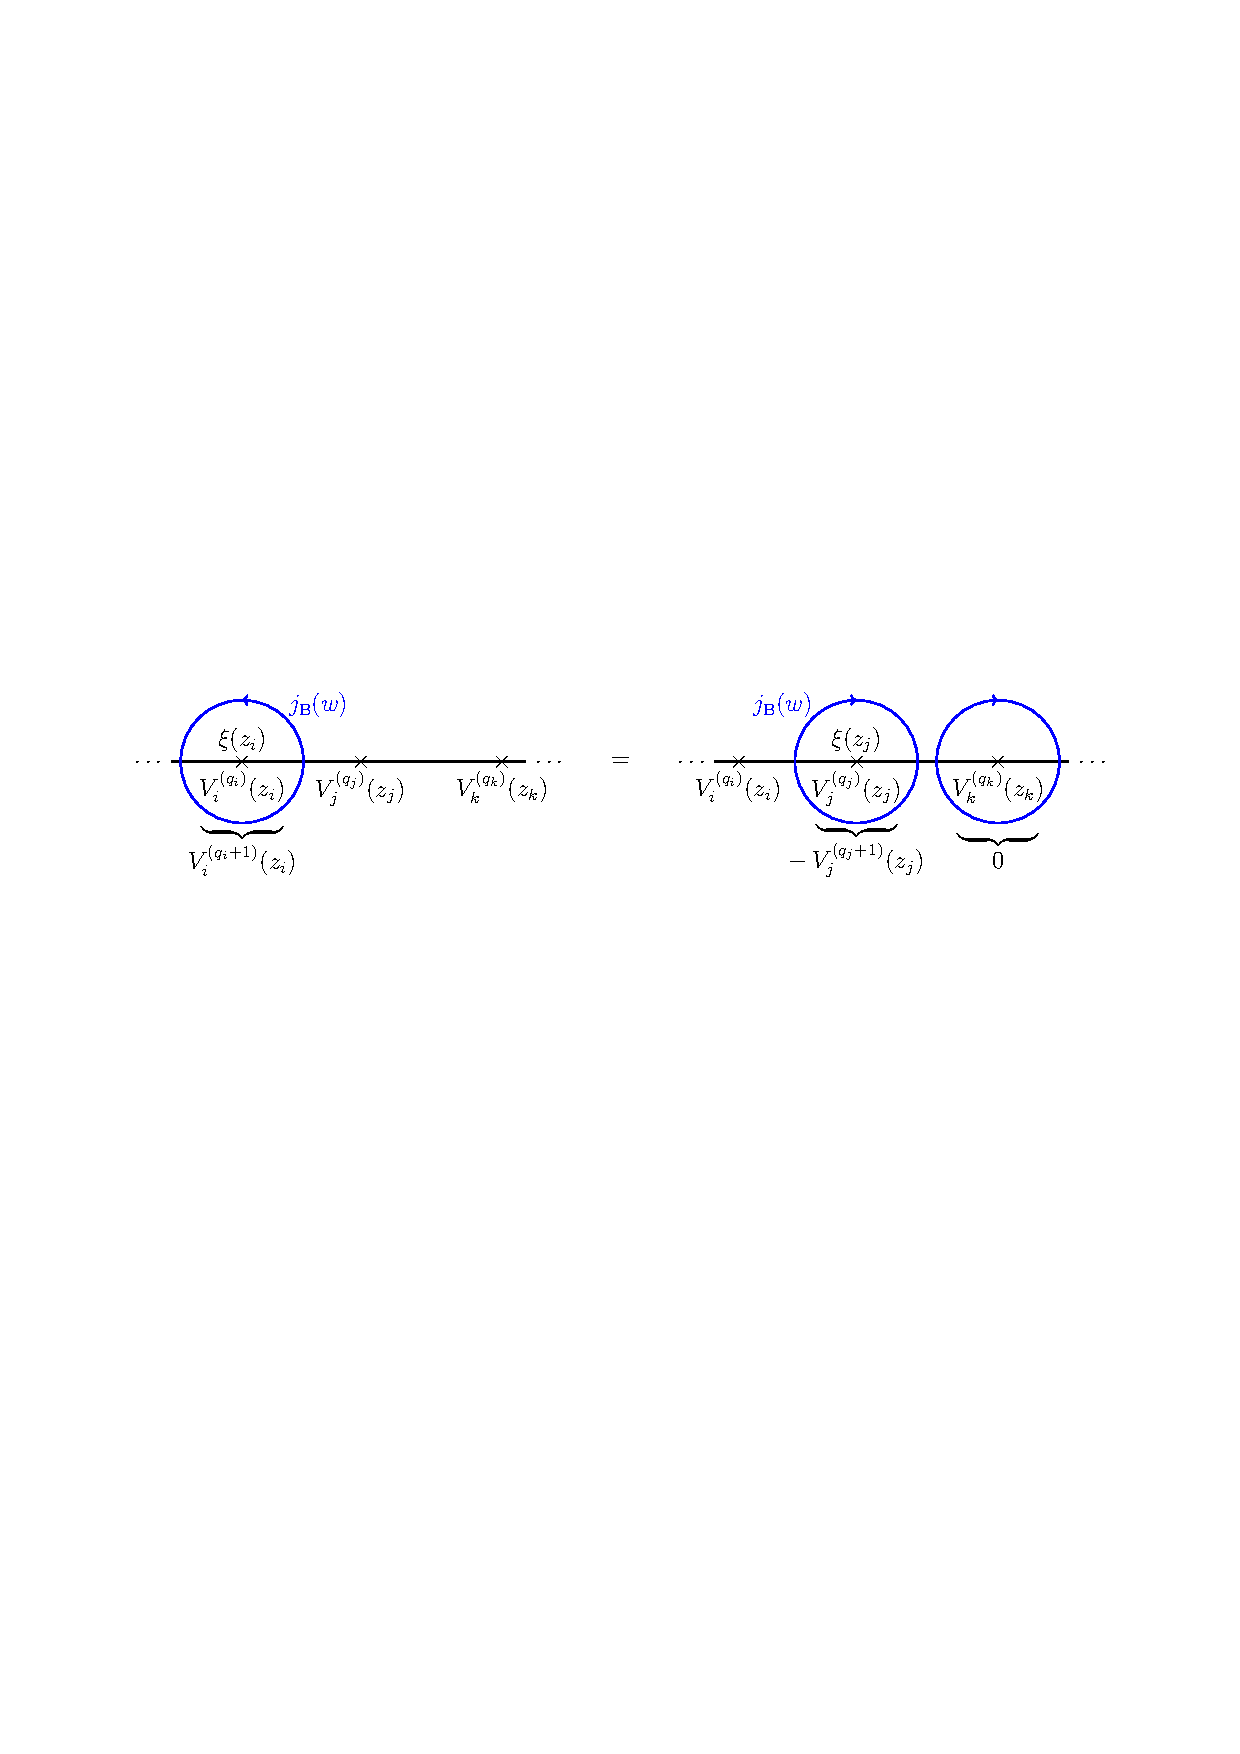
\includegraphics[width=\linewidth]{figs/fig2.pdf}
	\caption{围道替换}
	\label{fig:2}
\end{figure}
\section{*弦理论之间的对偶关系}
